\documentclass[10pt]{beamer}

\usepackage{../macros}

\title{Nombres réels approchés}

\hypersetup{
  pdftitle =  {Nombres réels approchés}
}

\begin{document}

\maketitle

%%%%%%%%%%%%%%%%%%%%%%%%%%%%%%%%%%%%%%%%%%%%%%%%%%%%%%%
\begin{frame}[fragile]
  \frametitle{Nombres réels approchés}
  Ou nombres réels inexacts. On parle de \alert{nombres flottants} (float).

  \begin{alertblock}{Calcul entier et réel en précision finie}
    Ils n'ont qu'un nombre limité de chiffres avant et après la ”virgule” (le point décimal).
  \end{alertblock}

%   %Rappel : le calcul \alert{entier} est exact,
%   \begin{lstlisting}
% > 1 %/% 2
% [1] 0
% > 1 / 2
% [1] 0.5
% > 2 / 3
% [1] 0.6666666666666666
%   \end{lstlisting}

  \begin{center}
    \alert{\textbf{Donc aucun nombre irrationnel !}}
  \end{center}

\begin{columns}[t]
\begin{column}{0.45\textwidth}
  \begin{exampleblock}{Approximation de $\pi$}
    \begin{lstlisting}[style=block]
> pi
[1] 3.141593
> sprintf('%.17f',pi)
[1] "3.14159265358979312"
> typeof(pi)
[1] "double"
\end{lstlisting}
Mais, $\pi = 3.141592653589793\mathbf{23}\ldots$
  \end{exampleblock}
\end{column}

\begin{column}{0.55\textwidth}
  \begin{exampleblock}{Approximation de $\sqrt 2$}
    \begin{lstlisting}[style=block]
> sqrt(2)
[1] 1.414214
> sprintf('%.17f',sqrt(2) ** 2)
[1] "2.00000000000000044"
> sqrt(2) ** 2 == 2
[1] FALSE
\end{lstlisting}
\end{exampleblock}
\end{column}
\end{columns}
\end{frame}


%%%%%%%%%%%%%%%%%%%%%%%%%%%%%%%%%%%%%%%%%%%%%%%%%%%%%%%

\begin{frame}[fragile]
  \frametitle{Nombres rationnels}
  Les nombres rationnels peuvent être représentés sous la forme d'une fraction, par exemple $\frac{1}{10}$.
  \begin{itemize}
  \item Le nombre $\frac{1}{10} = (0.1)_{10}$, par exemple, est simple dans le système décimal.
  \item Mais, il possède une infinité de chiffres après la virgule dans le système binaire !
    \[0.0001100110011001100110011001100110011001100110011\ldots\]
  \end{itemize}
  Lorsque R affiche une valeur approchée, ce n'est qu'une approximation de la véritable valeur interne de la machine :
  \begin{lstlisting}
> 0.1 # quelle est la valeur de 0.1 ?
[1] 0.1 # ceci est une illusion !
\end{lstlisting}

La fonction \texttt{print} ou \texttt{printf} permet de voir (en décimal) la véritable représentation en machine de 0.1 qui n'est pas 0.1 mais :
\begin{lstlisting}
> print(0.1,digits=17)
[1] 0.10000000000000001
\end{lstlisting}
\end{frame}

%%%%%%%%%%%%%%%%%%%%%%%%%%%%%%%%%%%%%%%%%%%%%%%%%%%%%%%
\begin{frame}[fragile]{Représentation des nombres réels}
  \begin{itemize}
  \item Les ressources d'un ordinateur étant limitées, on représente seulement un \alert{sous-ensemble des réels de cardinal fini}.
  \item Ces éléments sont appelés \alert{nombres à virgule flottante}.
  \item<alert@1> Leurs propriétés sont différentes de celles des réels.
  \end{itemize}

  \begin{alertblock}{Problèmes et limitations}
    \begin{itemize}
    \item Les nombres et les calculs sont nécessairement arrondis.
    \item Il y a des erreurs d’arrondi et de précision.
    \item On ne peut plus faire les opérations de façon transparente.
    \item L'ordre des opérations peut changer les résultats.
  \end{itemize}
\end{alertblock}


\begin{exampleblock}{Le zéro n'est plus unique !}
\begin{lstlisting}[style=block]
> 10^20 + 1 == 10^20
[1] TRUE
> 10^20 + 2 == 10^20
[1] TRUE
\end{lstlisting}
En math, il existe un unique nombre $y$ tel que $x + y = x$, le zéro !
\end{exampleblock}
\end{frame}

%%%%%%%%%%%%%%%%%%%%%%%%%%%%%%%%%%%%%%%%%%%%%%%%%%%%%%%

\begin{frame}[fragile]
  \frametitle{Égalité entre nombres flottants}
  Le calcul sur des nombres approchés étant par définition \alert{INEXACT}, on évitera sous peine de surprises désagréables de questionner l'\alert{ÉGALITÉ} en présence de nombres approchés !
  \begin{lstlisting}
> 0.1 + 0.1 + 0.1 + 0.1 + 0.1 + 0.1 + 0.1 == 0.7
[1] TRUE
> 0.1 * 7 == 0.7
[1] FALSE
> 0.1 + 0.1 + 0.1 == 0.3
[1] FALSE
> 0.1 * 3 == 0.3
[1] FALSE
\end{lstlisting}

Le domaine du calcul approché est TRÈS difficile, et prévoir à l'avance le nombre exact de décimales correctes lors d'un résultat de calcul reste réservé aux spécialistes d'analyse numérique (brrr) \dots

\begin{block}{Alors que faire ? Remplacer l'égalité par une précision h}
\begin{columns}[t]
\begin{column}{0.48\textwidth}
  \begin{lstlisting}[style=editor]
a == b # BAD !
  \end{lstlisting}
\end{column}
\begin{column}{0.48\textwidth}
  \begin{lstlisting}[style=editor]
abs(a - b) < h # GOOD !
  \end{lstlisting}
\end{column}
\end{columns}
\end{block}
\end{frame}

%%%%%%%%%%%%%%%%%%%%%%%%%%%%%%%%%%%%%%%%%%%%%%%%%%%%%%%
\begin{frame}[fragile]
  \frametitle{Autres problèmes avec les nombres flottants}


  \begin{exampleblock}{Une boucle infinie ?}
  \begin{lstlisting}[style=edblock]
x <- 1
while( x > 0 ) {
  print(x)
  x <- x / 2
}
\end{lstlisting}
Est-ce que cette boucle s'arrête ? En math ? En info ?
\end{exampleblock}


\begin{exampleblock}{Annulation catastrophique $x^2 - y^2$}
  \begin{lstlisting}[style=block]
> y <- 2**50
> x <- y + 1
> z1 <- x**2 - y**2 # appliquer directement la formule
> z2 <- (x - y)*(x + y) # appliquer une identité remarquable
> z2 - z1 # Est-ce que les résultats sont identiques ?
[1] 1
  \end{lstlisting}
\end{exampleblock}

\end{frame}



%%%%%%%%%%%%%%%%%%%%%%%%%%%%%%%%%%%%%%%%%%%%%%%%%%%%%%%
\begin{frame}
  \frametitle{Exemple : approximation de $\sqrt{r}$}
  Par la méthode des tangentes de Newton (1669).

  Soit à calculer la racine carrée approchée d'un nombre réel $\mathtt{r} > 0$, par exemple $\sqrt{2}$, sans utiliser \texttt{sqrt} !

  \begin{block}{Newton}
  Si $a$ est une approximation de $\sqrt{r}$ alors :
  \[
    b = \frac{1}{2}(a + \frac{r}{a})
  \]
  est une approximation encore meilleure ! Pourquoi ? Cf TD.
  \end{block}
  Nous allons développer cet algorithme en répondant à trois questions :
  \begin{description}
  \item[ITÉRATION] Comment améliorer l'approximation courante ?
  \item[TERMINAISON] Mon approximation courante $\mathtt{a}$ est-elle assez bonne ?
  \item[INITIALISATION] Comment initialiser la première approximation ?
  \end{description}
\end{frame}

%%%%%%%%%%%%%%%%%%%%%%%%%%%%%%%%%%%%%%%%%%%%%%%%%%%%%%%
\begin{frame}[fragile]
  \frametitle{Algorithme d'approximation de $\sqrt{r}$}
  \begin{block}{ITÉRATION}
    Pour \alert{améliorer} l'approximation, il suffit d'appliquer la formule de Newton, qui fait approcher $\mathtt{a}$ de $\sqrt{r}$ :
    \begin{lstlisting}[style=editor]
a = 0.5 * (a + r / a)
    \end{lstlisting}
  \end{block}

  \begin{block}{TERMINAISON}
  Mon approximation courante a est-elle \alert{assez bonne} ? Elle est assez bonne lorsque $\mathtt{a}$ est très proche de $\sqrt{r}$.
Notons $\mathtt{h}$ la variable dénotant la précision, par exemple $\mathtt{h} = 2^{-20}$.
\begin{lstlisting}[style=editor]
abs(a*a - r) < h
\end{lstlisting}
\end{block}
\begin{block}{INITIALISATION}
  Comment \alert{initialiser} l'approximation ? En fait, les maths sous-jacentes à la technique de Newton montrent que n'importe quel réel $\mathtt{a} > 0$ convient :
  \begin{lstlisting}[style=editor]
a = 1
  \end{lstlisting}
\end{block}
\end{frame}

%%%%%%%%%%%%%%%%%%%%%%%%%%%%%%%%%%%%%%%%%%%%%%%%%%%%%%%
\begin{frame}[fragile]
  \frametitle{Programme d'approximation de $\sqrt{r}$}
  \begin{lstlisting}[style=editor]
Racine <- function(r, h = 2**(-10)) {
  a <- 1
  while( abs(a*a -r) >= h) {
    print(a)
    a <- 0.5 * (a + r/a)
  }
  return(a)
}
\end{lstlisting}

\begin{lstlisting}
> approx <- Racine(r = 2, h = 10**(-10))
[1] 1
[1] 1.5
[1] 1.416667
[1] 1.414216
> print(approx, digit = 15)
[1] 1.41421356237469
> print(sqrt(2), digit = 15)
[1] 1.4142135623731
\end{lstlisting}

\begin{block}{Observation}
  La méthode de Newton converge rapidement vers le résultat.
\end{block}
\end{frame}

%%%%%%%%%%%%%%%%%%%%%%%%%%%%%%%%%%%%%%%%%%%%%%%%%%%%%%%
\begin{frame}
  \frametitle{Mais d'où vient la formule de Newton  $b = \frac{1}{2}(a + \frac{r}{a})$ ?}

  D'un simple calcul de tangentes (cf TD ou \href{https://fr.wikipedia.org/wiki/M\%C3\%A9thode\_de\_Newton}{wikipedia}) \dots

  \begin{center}
    \begin{tikzpicture}[xscale=3, yscale=2]
      \clip (0.5, -1.1) rectangle (3.1, 2.1);
      \draw[red,thick] (0,-2)  parabola (2,2);
      \draw[loosely dotted] (1, -1) grid (2,2);

      \node[red, thick, right] at (1, -1) {$y=x^2 - 2$};

      \draw[->] (1,0) -- (2.1, 0);
      \foreach \x in {1, 2}
      \draw (\x,1pt) -- (\x,-3pt)  node[anchor=north, right] {$\x$};

      \draw[->] (1,-2) -- (1,2.1);
      \foreach \y/\ytext in {-2, -1, 0, 1, 2}
      \draw (1,\y) -- (0.95,\y) node[anchor=east] {$\ytext$};

      \draw[thick] (2,2) -- (1.5, 0) node[above right] {$y=4x - 6$};;
      \fill (2,2) circle[radius=1.5pt, xscale=2/3];
      \fill (1.5,0) circle[radius=1.5pt,xscale=2/3];
    \end{tikzpicture}
  \end{center}
\end{frame}



%%%%%%%%%%%%%%%%%%%%%%%%%%%%%%%%%%%%%%%%%%%%%%%%%%%%%%%
 \questionSlide

%%%%%%%%%%%%%%%%%%%%%%%%%%%%%%%%%%%%%%%%%%%%%%%%%%%%%%%
 \appendix
 \backupSlides
%%%%%%%%%%%%%%%%%%%%%%%%%%%%%%%%%%%%%%%%%%%%%%%%%%%%%%%


 %%%%%%%%%%%%%%%%%%%%%%%%%%%%%%%%%%%%%%%%%%%%%%%%%%%%%%%
\begin{frame}{Répartition de flottants 6 bits sur la droite réelle}

\begin{columns}[t]
  \begin{column}{0.48\textwidth}
    \begin{block}{Flottant $\sim$ Notation scientifique}
      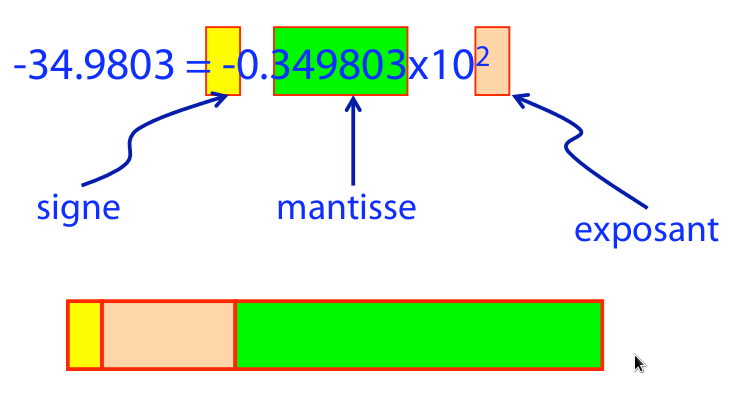
\includegraphics[width=\textwidth]{float-encoding}
    \end{block}
  \end{column}
  \begin{column}{0.48\textwidth}
    \begin{block}{Flottants sur 6 bits}
      Soit $2^6$ valeurs distinctes.
      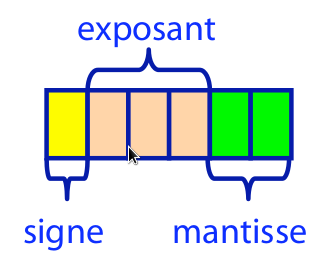
\includegraphics[width=3cm]{float-6bits-encoding}
    \end{block}
  \end{column}
\end{columns}

\begin{figure}[b]
  \centering
  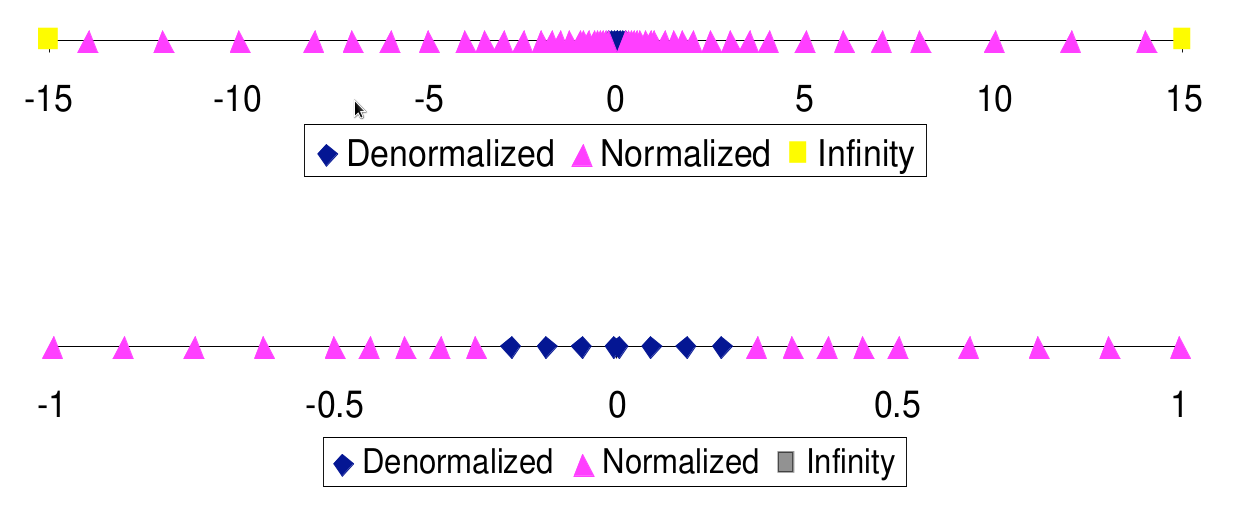
\includegraphics[width=0.9\textwidth]{float-6bits-distribution}
\end{figure}

\end{frame}

%%%%%%%%%%%%%%%%%%%%%%%%%%%%%%%%%%%%%%%%%%%%%%%%%%%
\begin{frame}{Tableau des flottants 6 bits}
  \begin{figure}[htbp]
    \centering
    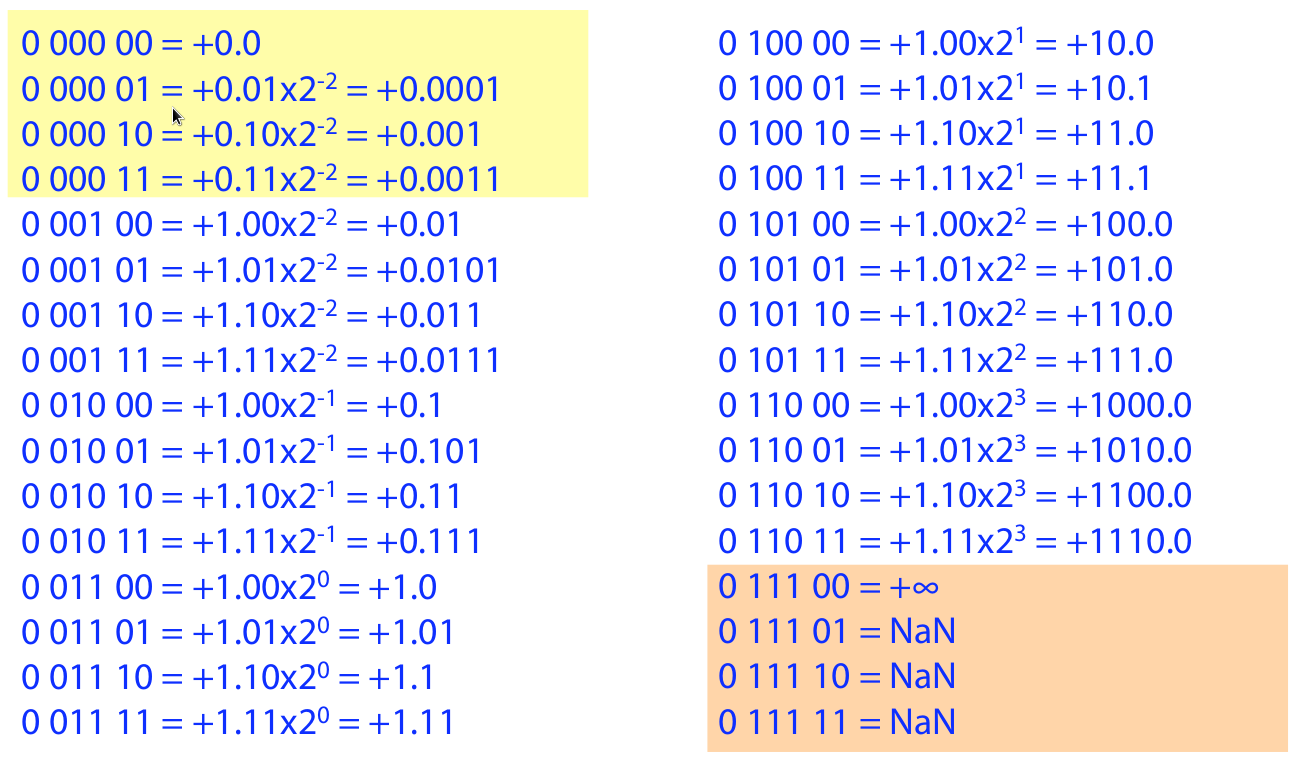
\includegraphics[width=\linewidth]{float-6bits-table}
  \end{figure}
\end{frame}

%%%%%%%%%%%%%%%%%%%%%%%%%%%%%%%%%%%%%%%%%%%%%%%%%%%
\begin{frame}{Quelques erreurs catastrophiques}
  \begin{itemize}
  \item En 1982  à la bourse de Vancouver, les calculs sur un indice nouveau, de valeur initiale 1000.0, sont tronqués (plutôt qu’arrondis). Après 22 mois la valeur calculée de l’indice est de 520 au lieu de 1098.892\dots
  \item Le 25 février 1991, à Dharan en Arabie Saoudite, un missile anti-missile Patriot américain rate l’interception d’un missile Scud irakien à cause d'une erreur d'arrondi dans sa trajectoire : 28 morts, plus d’une centaine de blessés.
%  \item Perte d’une plate-forme pétrolière en mer du Nord, au large de la Norvège, le 23 août 1991 (problème matériel + imprécision éléments finis) : coût estimé à 700 M\$.
  \item Lors des élections dans le Schleswig-Holstein le 5 avril 1992, l’affichage du pourcentage de voix des Verts sans décimales puis avec deux décimales change le résultat et donne la majorité au SPD au parlement allemand.
  \item Le 4 juin 1996, lors de son premier vol, la fusée européenne Ariane 5 explose 30 secondes après son décollage à cause d'une erreur d'\textit{overflow} dans l'ordinateur de bord causant une perte estimée à 500 M\$ (et 7 milliards de dollars d’investissement).
\end{itemize}

\end{frame}

%%%%%%%%%%%%%%%%%%%%%%%%%%%%%%%%%%%%%%%%%%%%%%%%%%%%%%%
% \begin{frame}[fragile]{Backup slides}
%   Sometimes, it is useful to add slides at the end of your presentation to
%   refer to during audience questions.

%   The best way to do this is to include the \verb|appendixnumberbeamer|
%   package in your preamble and call \verb|\appendix| before your backup slides.

%   will automatically turn off slide numbering and progress bars for
%   slides in the appendix.
% \end{frame}


%%%%%%%%%%%%%%%%%%%%%%%%%%%%%%%%%%%%%%%%%%%%%%%%%%%%%%%
% \begin{frame}[allowframebreaks]{References}

%   % \bibliography{../bib_parallelism,../bib_others}
%   % \bibliographystyle{abbrv}

% \end{frame}

\end{document}

%%% Local Variables:
%%% mode: latex
%%% TeX-master: t
%%% End:
